% Chapter 2

\chapter{Results and Discussions} % Write in your own chapter title
\label{Chapter5}
\lhead{Chapter 5. \emph{Results and Discussions}} % Write in your own chapter title to set the page header

As we have  to predict the indoor location of the user, we gathered our dataset by capturing RSSI fingerprints using our data capturing application which we further use to train our machine learning model.To train our machine learning model, we use three different machine learning algorithms. Firstly knn, which we used for supervised machine learning problem i.e.multiclassification problem. After tuning hyper-parameters of knn, it gives us accuracy of 90.04 while measuring Euclidean distance and of 90.03 while measuring Manhattan distance as shown in the Figure 5.1. 
\begin{figure}[h]
\begin{center}
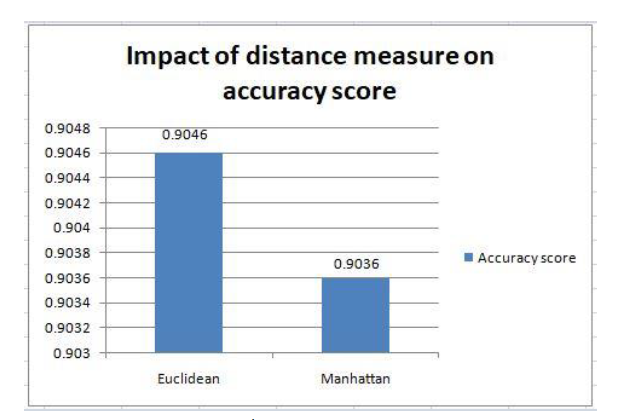
\includegraphics[scale=0.78]{dis}
\caption{Impact of distance measure on accuracy score}
\label{fig:1}
\end{center}
\end{figure}
Secondly, we choose random forest algorithm which works on the principle of random creation of decision trees and gives the final prediction by polling the score of all decision trees for multiclassification problems. We tuned random forest algorithm on different hyper-parameters i.e. number of decision trees, maximum number of splits and nodes. The best combination of setting these parameters gives us the trainng accuracy of 95.33 and testing accuracy of 90.1. The imapct of different number of trees  is shown in the Figure 5.2. 

\begin{figure}[h]
\begin{center}
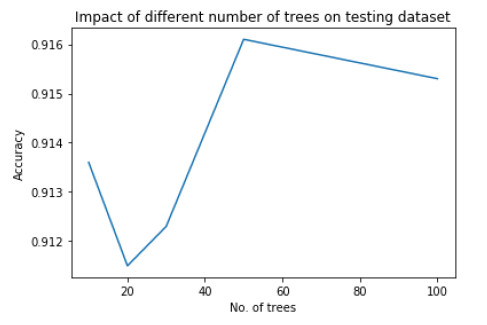
\includegraphics[scale=0.9]{rftree}
\caption{Impact of different number of trees on testing dataset}
\label{fig:2}
\end{center}
\end{figure}


For the better prediction of the indoor location of the user, we thirdly use neural networks in which we use 2-layered neural network for our multi-classification problem.The input layer consists of input neurons. Those neurons transmit data to the next layer, which in turn sends the output neurons to the output layer. To implement this algorithm, we have to find the best values for parameters at which accuracy score is maximum. For this purpose, we use GridsearchCV function to test for all possible combinations. Here are the results of impact of optimizations algorithms on accuracy score.

\begin{figure}[h]
\begin{center}
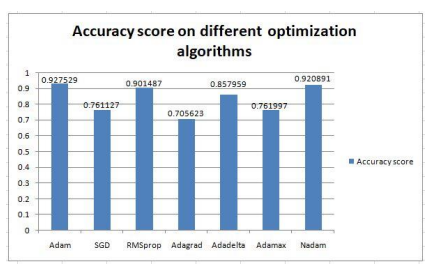
\includegraphics[scale=1.0]{optalgos}
\caption{Accuracy score on different optimization algorithms}
\label{fig:3}
\end{center}
\end{figure}

We also tune activation functions { 'relu', 'tanh', 'sigmoid', ‘linear’}. All of them gave same accuracy score.Hence, after checking the impact of choosing different values of parameters on accuracy score, we find out that best combination has following values:
\begin{itemize}
\item Batch size: 40
\item Epochs: 250
\item Optimization Algorithm: ‘Adam’
\item Weight Initialization Methods: ‘uniform’
\item Activation Function: ‘relu’ for hidden layer and ‘sigmoid’ for output layer
\item Number of Neurons for hidden layer: 27
\end{itemize}
So,we conclude that on the basis of accuracy, precision and recall score for k-NN, Random forest and ANN. It is clear that ANN has highest accuracy, precision and recall score. Hence, ANN is our selected mode.
\pagebreak

\section{Graphs}

The  accuracy, precision and recall graph of knn is as follows:
\begin{figure}[h]
  		\centering
    		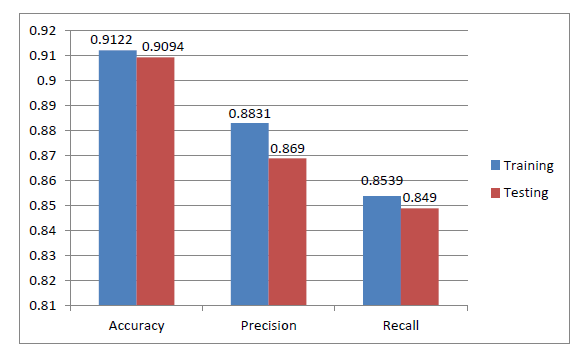
\includegraphics[scale=0.85]{./Figures/knncmgraph}
\caption{Accuracy, precision and recall graph of knn on training and testing sets}
\label{fig:4}
 		\end{figure}

The  accuracy, precision and recall graph of ann is as follows:

\begin{figure}[h]
  		\centering
    		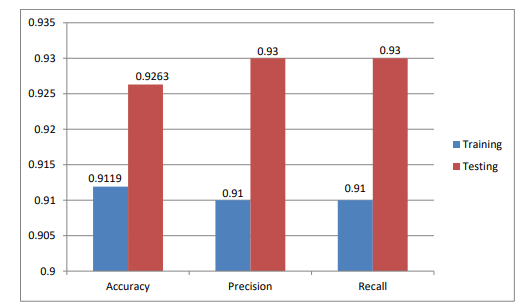
\includegraphics[scale=0.9]{./Figures/cmgraph}
\caption{Accuracy, precision and recall graph of ann on training and testing sets}
\label{fig:5}
 		\end{figure}

\pagebreak
\section{Confusion Matrix}

For the better prediction of the algorithms, we draw confusion matrix of the algorithims. The confusion matrix for knn is shown in the Figure(a) . As it is a multi-classification problem, it is a little bit different from binary classification. For example: ‘L1’ row shows that out of total samples in test data where data is labeled as ‘L1’, 92 instances were correctly classify, while 4 samples were wrongly predicted as ‘L9’.
\\\\
\begin{figure}[h]

  		\centering
    		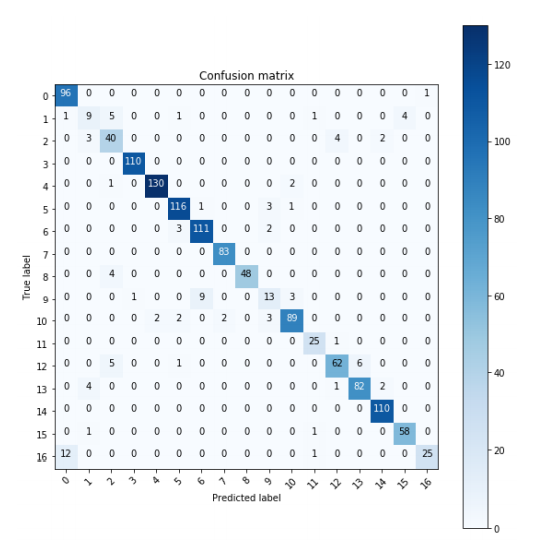
\includegraphics[scale=0.7]{./Figures/cm}
\caption{Confusion matrix for the evaluation of knn}
\label{fig:6}
 		\end{figure}


The confusion matrix for ann algorithm is shown in the Figure(b). As we use label encoder, so it encode classes ranges from 0 to 16. Here is the actual sequence, it means ‘L1’ encode to 0, ‘L10’ encode to 1 and so on:
\\\\
%['L1','L10','L11','L12','L13','L15','L16','L19','L2','L20','L21','L3','L4','L5','L6','L8','L9']
\begin{figure}[h]

  		\centering
    		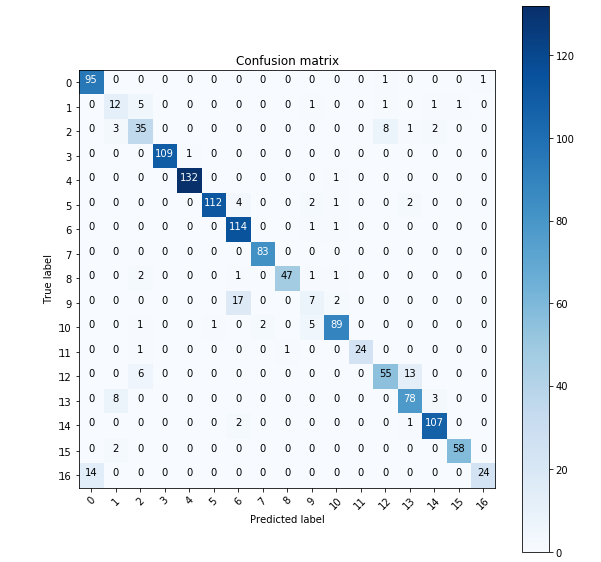
\includegraphics[scale=0.7]{./Figures/cmann}
\caption{Confusion matrix for the evaluation of ann}
\label{fig:7}
 		\end{figure}


